\chapter{Data Review}

In this chapter we take a deeper look into the data and the process of collecting, translating, and encoding the data. Our partner has provided a small sample of 1000 labeled data points. This data was manually labeled by an human annotator. 

\section{Overview}

The data consists of a merchant name, merchant website (url), merchant category, and merchant tag as shown in Table \ref{tab:data_point}. 

\begin{table}[h]
\begin{tabular}{|l|l|l|l|}
\hline
merchant name            & merchant url            & merchant category & merchant tags           \\ \hline
State Hospital & http://hospital.com/ & Health   & '\{"Clinic"\}' \\ \hline
\end{tabular}
\caption{This is an example of a single data point from the original data set.}
\label{tab:data_point}
\end{table}


The current process consists of giving the merchant url to an annotator and the annotator then views the website and either can instantly  provide a label and tags for the website or in some cases may need to browse further into the website (by viewing sibling pages such as the 'About Us' sections or product pages) to get an idea of how the website should be classified. 

The merchant tags are ordered by specificity, with the first tag in the list being the most general and the final being the most specific. An example of the tag hierarchy is show in Table. \ref{tab:tags} where we can see that this sample consists of data from various categories all contained within the 'Eco' side tag grouping.


\begin{table}[h]
\begin{tabular}{|l|l|l|l|l|}
\hline
Category    & Level 1 Tag           & Level 2 Tag        & Level 3 Tag  & Side Tag \\ \hline
Travel      & Local Transport       & Micro-mobility     & Bike Sharing & Eco      \\ \hline
            &                       & Public Transport   &              & Eco      \\ \hline
Fashion     & Clothing - Other      & Second Hand        &              & Eco      \\ \hline
Car         & Charging Station      &                    &              & Eco      \\ \hline
            & Car Sharing           &                    &              & Eco      \\ \hline
\end{tabular}
\caption{This is an example of how the tags use different levels.}
\label{tab:tags}
\end{table}

The tags are important because they allow us to separate the data even further and group/ sort the data differently. However, in our work we didn't opt to use the tags at this time.

\section{Collection}

Similarly to the annotator our goal is to automate the navigation, collection/ storing process, and classification of the website. This pipeline speeds up the browsing process and can allow the annotator to spend much less time annotating and require the annotator to only annotate data expected to drastically improve the classifier.

The initial 1000 data points we received were labels with a pointer (a url) to where the text data is located. The labels needed the text from the websites that the annotator viewed to begin the classifying process. To gather the text data from the websites we used the Scrapy framework to extract text data from a single top level page of a website. We chose only to scrape the top level (main or home) page text because of the results published in another study where it was observed that adding more pages to the data set does not necessarily mean obtaining better results (\cite{sahid2019ecommerce}). 

Out of these initial data points 179 contained links that could not be accessed or links that provided no text data that could be scraped. Out of the remaining 821 data points 274 of them were in English. Out of the remaining 274 English data points the data was distributed into the categories as shown in Figure \ref{fig:original_english_counts}.

\section{Processing}

It is important for us to have the data in English as it allows us to exploit stop words when using the Scikit-Learn TF-IDF vectorizer to construct our data set. Stop words are words like “and”, “the”, “him”, which are presumed to be uninformative in representing the content of a text, and which may be removed to avoid them being construed as signal for prediction (\cite{sklearn62feature}). This holds true for our data set as well.

At this stage, it was clear that our data set wasn't representing all categories equally. The 'Food and Drink' category has many more data points then the 'Culture' and 'Investments' categories which each had a single data point, see Figure \ref{fig:original_english_counts}. The 'Children' and 'Financial Services' categories weren't represented at all. Obviously this was problematic because we would like to have, minimum, three data points in each category to build train and test sets.

\begin{figure}[!ht]
  \centering
  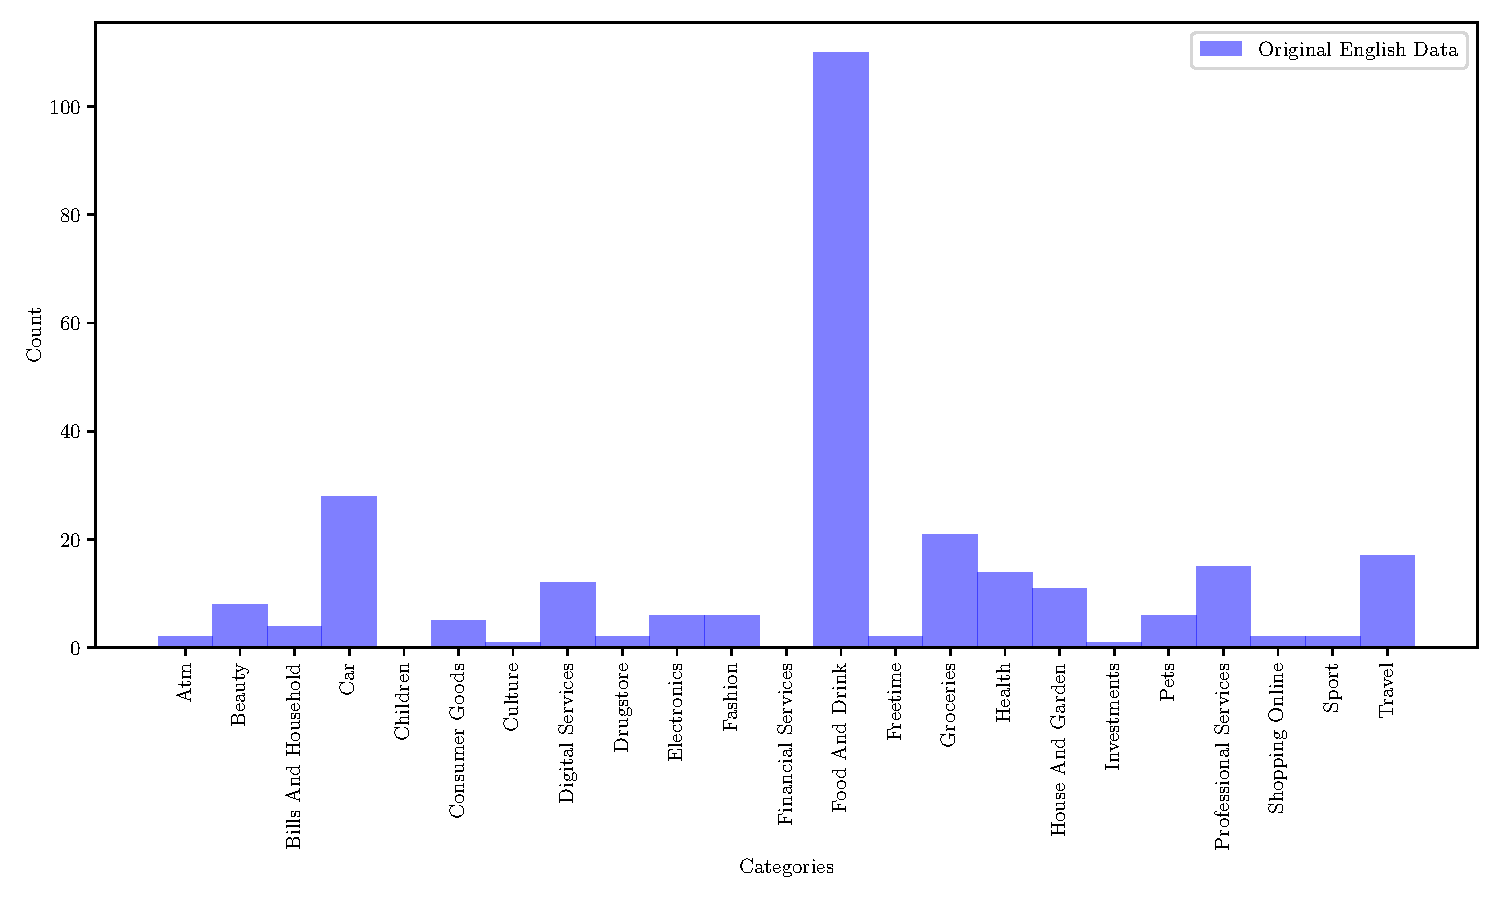
\includegraphics[width=\textwidth]{../img/plot_original_english_counts.pdf}
  \caption{The histograms for the original usable english data.}
  \label{fig:original_english_counts}
\end{figure}

At this point we had a significant amount of data that wasn't being used (the untranslated data). We decided to find a way to translate the existing data. We tried various libraries available on GitHub but weren't getting good results. We found that Azure had a service available and a free option of up to 2 million characters translated per month. This was a viable option and we were able to use this API to translate the remaining data. We limited the number of characters to 1000 per data point from the scraped text to avoid maxing out the API.

An example of the first 100 characters of raw scraped text data from a website is shown in Table \ref{tab:text_examples}. The scraped text data is a single string of text that is a concatenation of all the text data pulled from the website url. 

\begin{table}[!ht]
\centering
\caption{Raw text collected by scraper and the translated text.}
\begin{tabular}{|l|p{10cm}|}
\hline
Raw & DentalVision - Profesionální soukromá zubní klinika v centru Hradce Králové ÚvodSlužby a ceníkOrdina \\ \hline
Translated & DentalVision Professional private dental clinic in the center of Hradec Králové IntroductionServices \\ \hline
\end{tabular}
\label{tab:text_examples}
\end{table}

We can see that the symbols were removed and the majority of the words were translated. There are still some issues with words being concatenated, but we attempt to break these words apart before passing the text to the TF-IDF vectorizer.

In addition to the original data we also manually collected and labeled 141 additional data points. All the original data and additional data counts are shown in Figure \ref{fig:all_hist} and discretely in Appendix Table \ref{tab:en_data_counts}.


\begin{figure}[!ht]
  \centering
  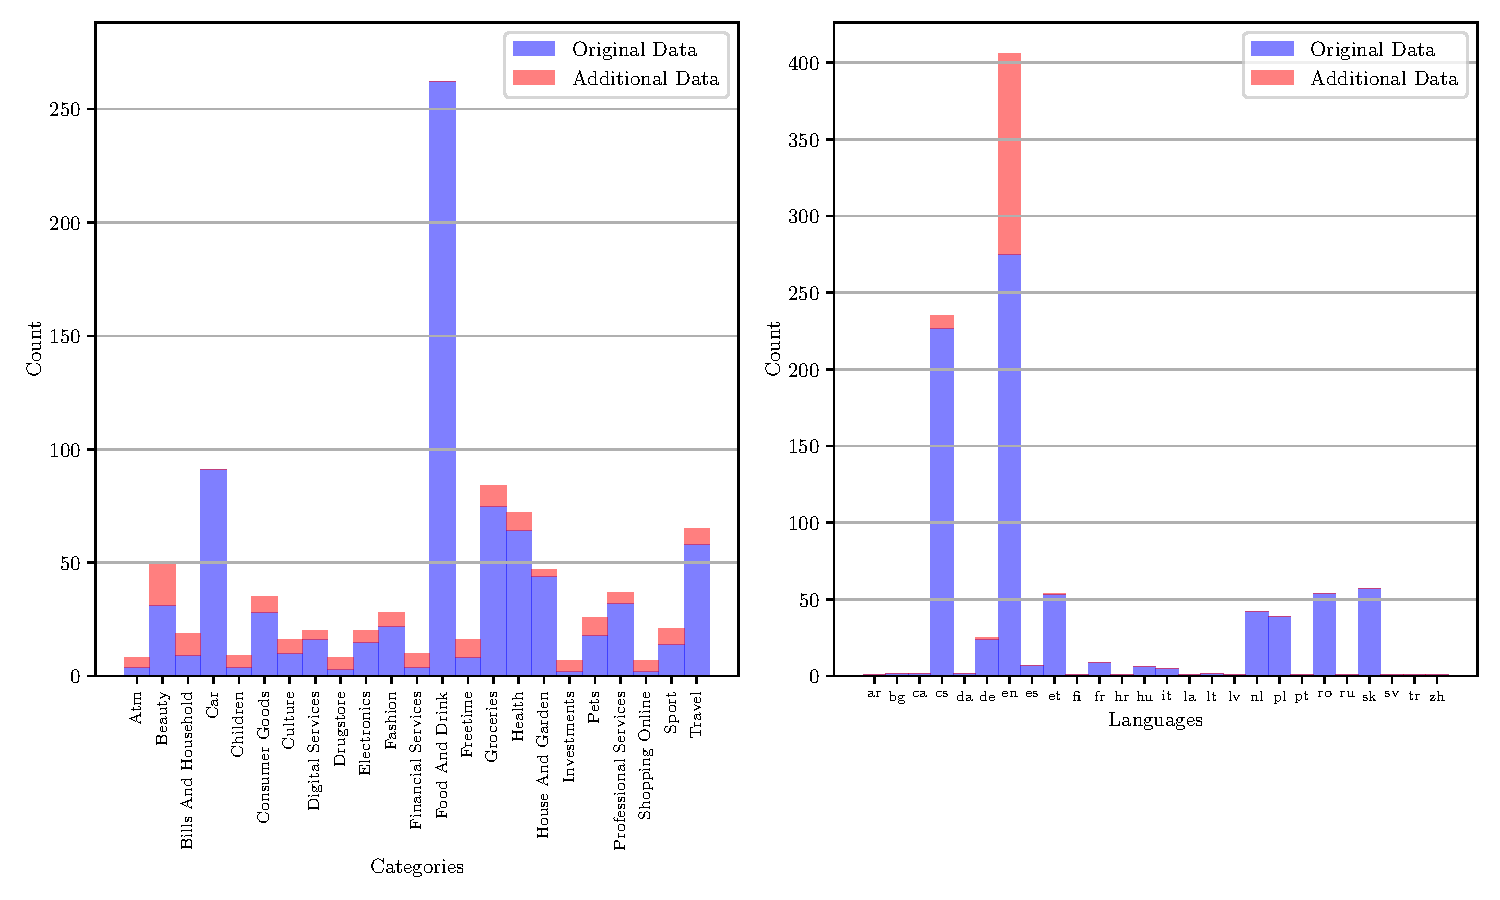
\includegraphics[width=\textwidth]{../img/plot_all_hist.pdf}
  \caption{The histograms for the original and additional data for all languages.}
  \label{fig:all_hist}
\end{figure}


After translating the data we used the TF-IDF vectorizer from Scikit-Learn. We were able to find highly correlated words for each category using Chi Squared analysis with only the original data, shown below in Table \ref{tab:correlated_unigrams_original}. Some categories such as 'Culture', 'Digital Services', 'Shopping Online' that have few data points have words such as 'kihnu', 'td', 'patria', respectively, which have no relative meaning to the category in English. 

From what we discussed in the previous section, we can see that the 'Culture' category has only one data point and the 'Digital Services' category has only two data points. This is problematic because if the single data point we have is doesn't represent the category well then we will continue to have difficulty classifying until we have more robust data.


\begin{table}[!ht]
\centering
\caption{Keywords from TF-IDF with Chi Squared using the original data.}
\begin{tabular}{llll}
\toprule
{} &       Keyword 1 &      Keyword 2 &   Keyword 3 \\
\midrule
Atm                   &         banking &    individuals &       caixa \\
Beauty                &    hairdressing &    hairdresser &        hair \\
Bills And Household   &         liberty &       internet &    fullness \\
Car                   &            cars &           auto &         car \\
Children              &             toy &           sold &     toysrus \\
Consumer Goods        &           kiosk &        flowers &      flower \\
Culture               &         theater &         museum &       kihnu \\
Digital Services      &          synnex &          bitly &     servers \\
Drugstore             &     esodrogeria &      detergent &     drimble \\
Electronics           &         laptops &          onoff &   computers \\
Fashion               &           rings &      jewellery &       women \\
Financial Services    &             pre &         nissan &   insurance \\
Food And Drink        &            cafe &            bar &  restaurant \\
Freetime              &  representation &         casino &      likely \\
Groceries             &          liquor &           maso &      bakery \\
Health                &            drug &         dental &    pharmacy \\
House And Garden      &       skylights &         paints &    hardware \\
Investments           &        mistakes &     investment &      patria \\
Pets                  &             mat &            pet &  veterinary \\
Professional Services &          toilet &        faculty &      parcel \\
Shopping Online       &           owner &        default &        joom \\
Sport                 &          adidas &      singltrek &  functional \\
Travel                &           rooms &  accommodation &       hotel \\
\bottomrule
\end{tabular}

\label{tab:correlated_unigrams_original}
\end{table}


We also calculated the variable importance using the RandomForestRegressor from Scikit-Learn and provided a list of the top 20 most important words from the TF-IDF vectorizer. This helps us orient ourselves within the data as well as check if there may be any anomalies. The list of top 20 most important words are shown in Appendix Table \ref{tab:top_20_words}.



